
\iffalse
Features  
\begin{itemize}
	\item Qualitative representation - states and transitions
	\item State identification services:
	\begin{itemize}
		\item State details and attribute highlighting - histograms + attribute colors
		\item \lstopar{Timeline + parallel coordinates \cite{parcoords} - when do states occur in time}
		\item \lstopar{Coloring states based on attributes}
		\item Decision trees + rule extraction - Explanation of states
		\item Automatic name generation
		\item Zooming into a state + showing paths from a state
	\end{itemize}
\end{itemize}
\fi

After registering, the user is presented with a dashboard, where they can organize their models.
If they wish to create a new model, they have to upload a CSV file with the dataset they would
like to visualize. They are then taken through a configuration form, where they select attributes,
clustering method, aggregation strategy and attributes used to model transitions. When completing
the form, their new model is constructed. The construction time varies depending on the size of 
their dataset and configuration. We present construction times in Section \ref{sec:implementation}.

Once constructed, a StreamStory model is displayed using a three panel user interface, an example of
which is shown in Figure \ref{fig:teaser} \lstopar{[TODO teaser reference not appearing]}. As mentioned
in Section \ref{sec:introduction}, we summarize the model in a qualitative manner using states and 
transitions, where we associate each state with a circle and each transition with an arrow on the 
central panel. The size of a state is calculated from the associated entry in the stationary distribution
and is proportional to the fraction of time the system spends in the state. The thickness of each arrow
is proportional to the associated transition probability. When using the model as a
monitoring tool, the current state (\lstopar{orange}) and the most likely future states (\lstopar{blue})
are highlighted. The current state is determined by assigning the current data point to its nearest 
centroid, as presented in Section \ref{sec:multiscale-implementation}, and is updated in real-time as
the data arrives into the system.

When first opening the user interface, the model is presented on a coerce scale with only a handful
of states. Users can then explore the model using by either traversing the scales using the zoom 
function, isolate and explore individual states using the "Zoom Into" function, \lstopar{or explore the 
graph as a tree using the "Show Path" function}.

A graph with states and transitions is not very informative by itself. Therefore we offer several 
visualization services assist users identifying the meaning of states. These range from automatic
state naming, state histograms, attribute highlighting and timeline histograms to decision trees
which visualize the states properties in a \lstopar{tree manner} and \lstopar{extracted rules}.
These services are shown when the user clicks on a state and thereby selects it and will be 
explained in the following subsections.

\subsection{Automatic Labeling}

Looking at graphs by itself is not very informative. Although representing the system as states and 
transitions gives insight into the dynamics of the system, it fails to provide a comprehensive summary 
of the dataset. \lstopar{Indeed, our experiments showed first time users were quite confused when viewing
our model with unlabeled states and had difficulty executing even the simplest tasks like finding
states with high temperature in example \ref{sec:experiments-weather}}.

To overcome this issue, an automatic, data-driven, naming service was added. The service labels
states based on the inner-state attribute distributions by concatenating the most outlying attribute
with a discrete level with values: lowest, low, high or highest. An example of an automatic label
is shown in Figure \ref{fig:example-naming}.

\begin{figure}[h!]
	\centering
	\label{fig:example-naming}
	\begin{subfigure}{.48\columnwidth}
	  	\centering
	  	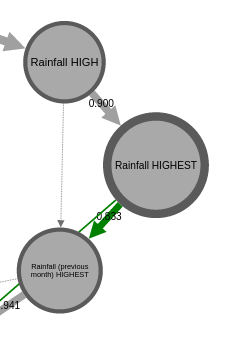
\includegraphics[width=0.7\columnwidth]{example-state-naming}
  		\caption{\lstopar{TODO}}
  		\label{fig:example-naming-label}
	\end{subfigure}
	\begin{subfigure}{.48\columnwidth}
	  	\centering
	  	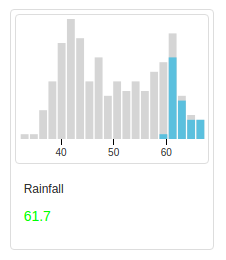
\includegraphics[width=\columnwidth]{example-state-naming-histogram}
	  	\caption{\lstopar{TODO}}
	  	\label{fig:example-naming-histogram}
	\end{subfigure}
\end{figure}


In order to assist the user in identifying the meaning of states, the system provides automatic default
state names, based on the distribution of attributes in the state. Each state is given a default name
by combining its most outstanding attribute with a discrete level: LOWEST, LOW, HIGH or
HIGHEST.

The attribute and the level are chosen by comparing its distribution inside the state to the global
distribution in all the states through histograms. This is achieved by first computing the percentiles
of the global distribution. The $40^{th}$ percentile is then computed for the state distribution and
compared against the global distribution. If this percentile lies below the $25^{th}$ or $12^{th}$
percentile, the state is marked with LOW or LOWEST respectively. The final name is chosen according
to the attribute which lies in the lowest percentile.

\subsection{Visual Assistance}

When a state becomes selected, the user interface presents the user with several visual aids which
assist them in identifying the states' meaning. The first of these aids is the timeline histogram
which shows the distribution of the states occurrence over time. An example is shown in Figure 
\ref{fig:time-hist}.

\begin{figure}[h!]
	\centering
	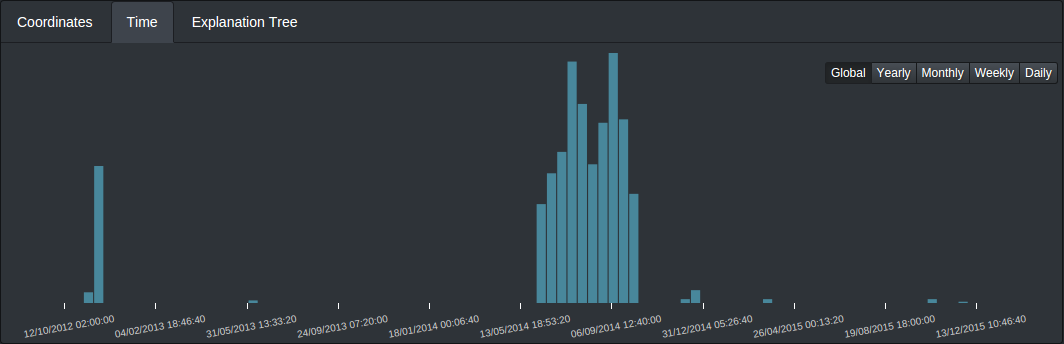
\includegraphics[width=\columnwidth]{timeline}
	\caption{[TODO example decision tree].}
	\label{fig:time-hist}
\end{figure}

[TODO histograms]




\subsection{Decision Trees and Rule Extraction}

An alternate description of a state is generated through the induction of decision trees. Decision
trees are classification models often used in domains such as medicine for their explanatory power.
When a decision tree is induced, a splitting attribute and cut value are chosen recursively by a
design time criteria. The user can then interpret the tree by traversing the path from the root 
to one of the leafs.

In our use case, we use decision trees as a tool for explaining states. We induce one tree for each
state by classifying the observations form the state against the observations of all other states
thus obtaining a qualitative description of the state. Figure \ref{fig:example-decision-tree} and
Figure \ref{fig:example-decision-tree-rule} show an example decision tree and extracted rules
from a state in the weather dataset presented in section \ref{sec:experiments-weather}.

\begin{figure}[h!]
	\centering
	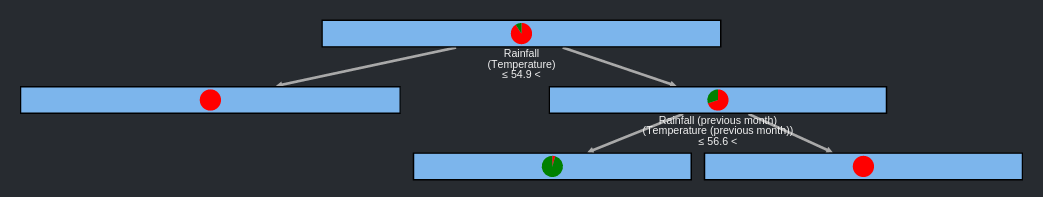
\includegraphics[width=\columnwidth]{tree-rainfall}
	\caption{[TODO example decision tree].}
	\label{fig:example-decision-tree}
\end{figure}

\begin{figure}[h!]
	\centering
	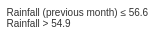
\includegraphics[width=100pt]{rule}
	\caption{[TODO rule generated from decision tree].}
	\label{fig:example-decision-tree-rule}
\end{figure}